
\appendix
\chapter{Appendix}

\section{Influence of Aperture}
\label{app:sec:ApertureInfluence}

The aperture \( D \) of a \gls{uca} is defined as
\[
    D = \frac{d_{\text{Ant}}}{\lambda_C} = \frac{f_C}{c_0} d_{\text{Ant}},
\]
has a significant impact on the array's performance~\cite{meyer,tuncer.ch2,tuncer.ch6}. It affects angular resolution,
directivity, sensitivity, and the operational frequency range. Specifically, a larger \( D \) enhances the system's
ability to resolve closely spaced sources, focus on specific directions, detect weak signals, and operate over a wider
frequency range. However, as demonstrated in~\cite[Chapter 8.3]{meyer}, an increased \( D \) also introduces more ambiguities
in the manifold, potentially reducing detection probability.

\section{General Form of a Covariance Matrix}
\label{app:sec:GeneralCovMatrix}
The covariance matrix, denoted as \( \bfm{C}_x \), is a crucial concept in statistical signal processing and machine
learning. It encapsulates the second-order statistics of a dataset, which comprise the means and variances of the
variables, as well as the covariances between each pair of variables.

\[
    \bfm{C}_x =
    \begin{bmatrix}
        \operatorname{Var}[x_1]    & \operatorname{Cov}[x_1, x_2] & \cdots & \operatorname{Cov}[x_1, x_n] \\
        \operatorname{Cov}[x_2, x_1] & \operatorname{Var}[x_2]    & \cdots & \operatorname{Cov}[x_2, x_n] \\
        \vdots            & \vdots            & \ddots & \vdots            \\
        \operatorname{Cov}[x_n, x_1] & \operatorname{Cov}[x_n, x_2] & \cdots & \operatorname{Var}[x_n]
    \end{bmatrix}
\]

The diagonal elements \( \sigma^2_{x_i} \) represent the variances of the respective variables \( x_i \).
The off-diagonal elements \( \sigma_{x_i, x_j} \) represent the covariances between each pair of variables
\( x_i \) and \( x_j \).

\section{Distribution of the noise eigenvalues}
\label{app:sec:NoiseEigvalDistrib}
\begin{figure}[H]
    \centering
    \subfloat[]{{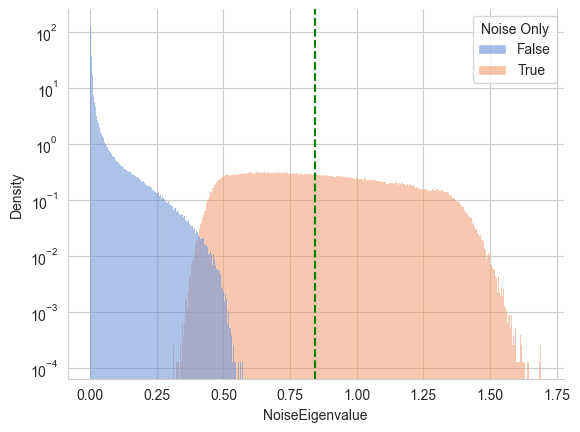
\includegraphics[width=0.5\textwidth]{figures/04_ModelOrderEstimation/noise_eigval_distrib.png}}}
    % \hspace{0.5cm}
    \subfloat[]{{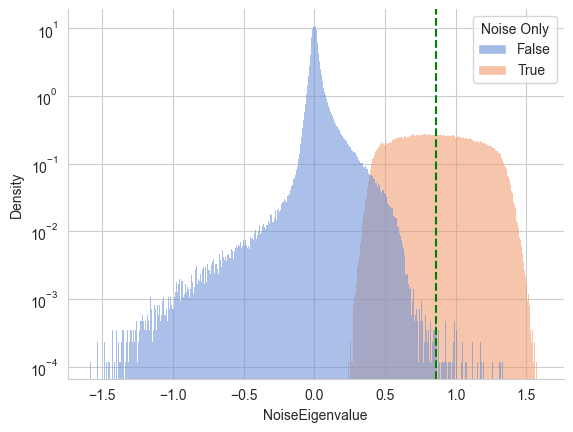
\includegraphics[width=0.5\textwidth]{figures/04_ModelOrderEstimation/noise_eigval_distrib_sub.png}}}
    \caption{Density estimates of noise eigenvalues of the full (a) and sub-sampled (b) covariance matrices, and \( K = 100 \).}
    \label{fig:noise_eigval_distrib}
\end{figure}

\autoref{fig:noise_eigval_distrib} depicts the density estimates of noise eigenvalues for both full and sub-sampled
covariance matrices, given a set number of snapshots \( K = 100 \).
The dataset was generated with a specified noise level of \( P_\eta = -120 \, \si{\deci\bel}_{(\si{\micro\volt})} \),
equating to a noise variance of \( \sigma^2_\eta = 1 \si{\micro\volt\squared} \). This baseline allows for an expectation
where noise eigenvalues ideally cluster around the noise variance as per the theoretical prediction (\autoref{eq:eigval_superimposed}).
In the noise-only case, where no signals are present (\( N = 0 \)), the orange distribution indeed aligns with this prediction.
However, the blue distribution, representing scenarios with one to five signals (\( N \in \{1, \ldots, 5\} \)), deviates
from this pattern.

\begin{figure}[H]
    \centering
    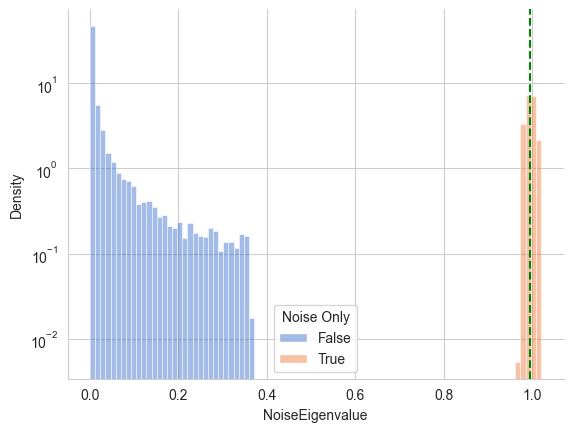
\includegraphics[width=0.45\textwidth]{figures/04_ModelOrderEstimation/noise_eigval_distrib_100k.png}
    \caption{Distribution of noise eigenvalues for \( K = 1e5 \).}
    \label{fig:noise_eigval_distrib_100k}
\end{figure}
Notably, with an increased snapshot count (\( K = 1e5 \)), depicted in \autoref{fig:noise_eigval_distrib_100k}, the
central tendency of the noise eigenvalues for \( N = 0 \) shifts closer to \( \sigma^2_\eta \) which is
in line with expectations. However, the separation between the two clusters—one corresponding to the noise-only case and
the other where signals are present— cannot be explained by the theoretical expectations.
One must consider whether this bifurcation is a characteristic of the data and model or, potentially a ``bug'', within
the Python environment used for analysis.


\section{Employed Boxplots}
\label{app:sec:Boxplot}

\begin{figure}[H]
    \centering
    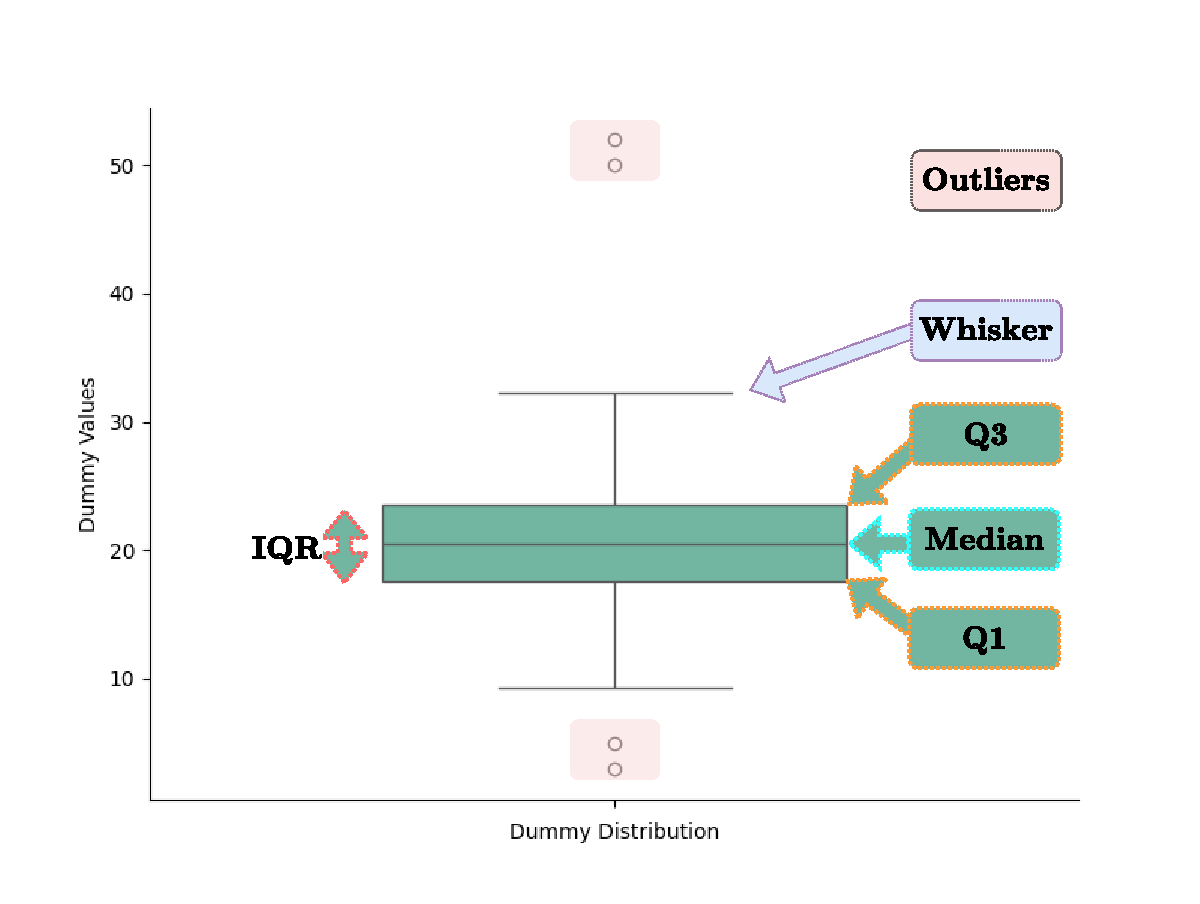
\includegraphics[width=0.7\textwidth]{figures/Appendix/boxplot.pdf}
    \caption{Visual explanation of a boxplot.}
    \label{fig:boxplot}
\end{figure}

\begin{itemize}
    \item \textbf{Middle Line:} Indicates the median, dividing the box into segments representing the middle 50\% data spread.
    \item \textbf{Box:} Represents the middle 50\% of the data, spanning from the first to the third quartile, enclosing the IQR.
    \item \textbf{Whiskers:} Extend to 1.5 times the interquartile range (IQR) from the quartiles, marking the data range. Points beyond are outliers.
\end{itemize}

\newpage{}

\section{Further Material on the Hyperparameter Optimization of the CNN}
\label{app:sec:FurtherCNN}

\subsubsection{Dropout Rate}
\begin{figure}[H]
    \centering
    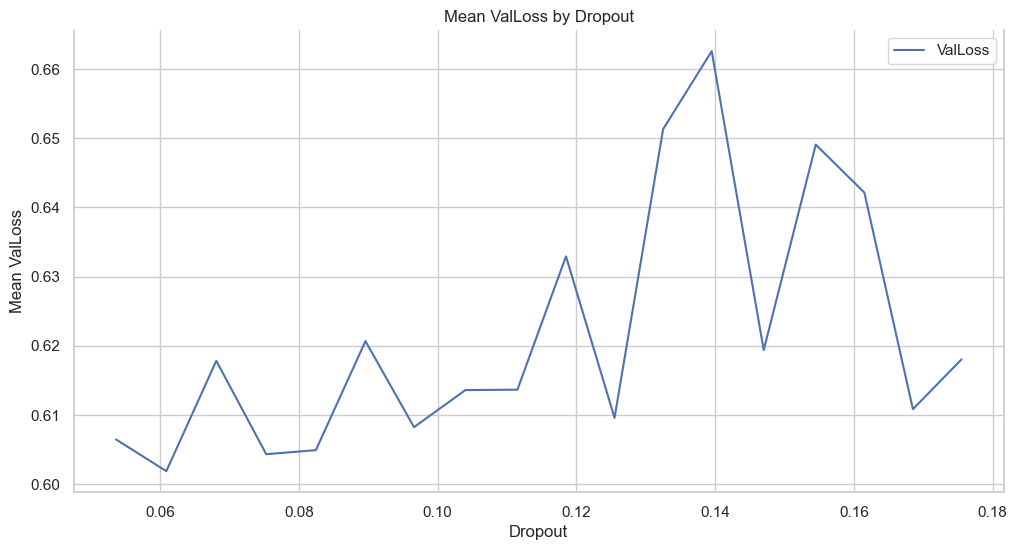
\includegraphics[width=0.6\textwidth]{figures/06_ModelExploration/4_CNN/dropout_274_18bins.png}
    \caption{Impact of the dropout rate on the validation loss \( \lossCEVal \).}
    \label{fig:dropout_cnn}
\end{figure}

\subsubsection{Learning Rate}

\begin{figure}[H]
    \centering
    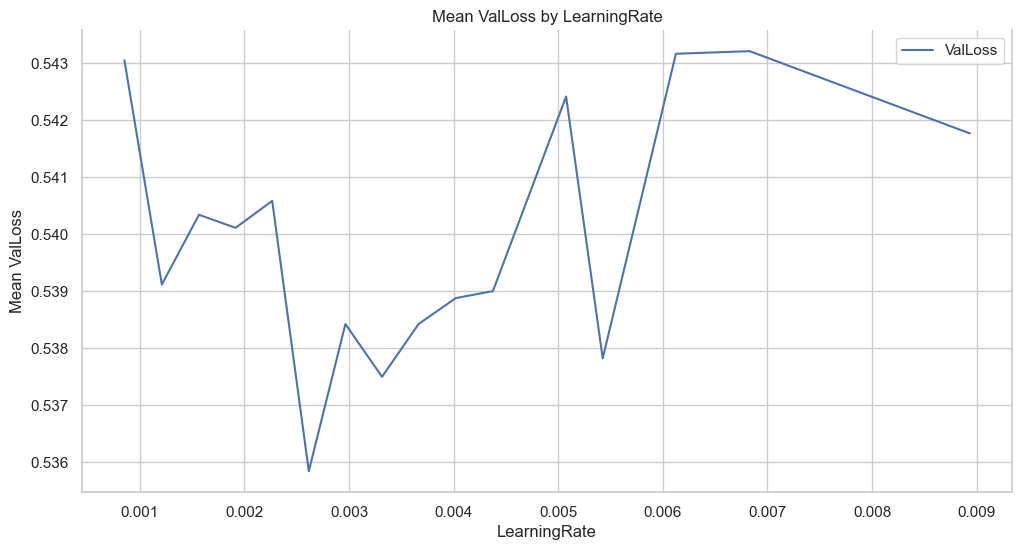
\includegraphics[width=0.6\textwidth]{figures/06_ModelExploration/4_CNN/learning_rate.png}
    \caption{Impact of the learning rate on the validation loss \( \lossCEVal \).}
    \label{fig:lr_cnn}
\end{figure}

While the local minimum of the validation loss \( \lossCEVal \) w.r.t.\ the learning rate was found to be at \( \gamma \approx 0.0026 \),
the learning rate for the final model was set to \( \gamma = 0.002 \) to account for the reduced batch size and longer training time.

\subsubsection{Weight Decay}

\begin{figure}[H]
    \centering
    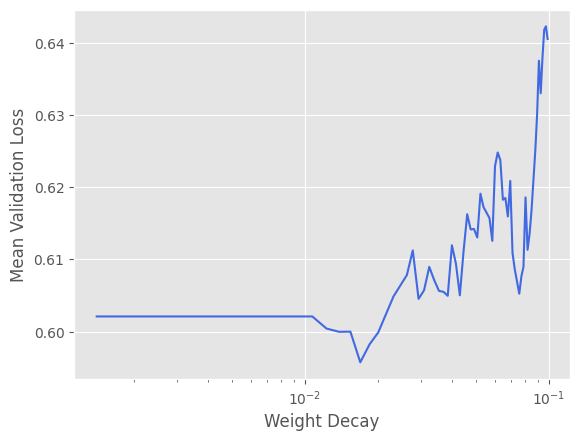
\includegraphics[width=0.6\textwidth]{figures/06_ModelExploration/4_CNN/conv_weighdecay_bin64_roll7_valloss.png}
    \caption{Impact of the weight decay on the validation loss \( \lossCEVal \).}
    \label{fig:wd_cnn}
\end{figure}
Additionally, to~\autoref{fig:wd_cnn} being created by binning the weight decay values into 64 bins, a rolling mean with
a window size of 7 was applied to the data.

\section{Further Material on the Hyperparameter Optimization of the RNN}
\label{app:sec:FurtherCNN}
\subsubsection{Learning Rate}
\begin{figure}[H]
    \centering
    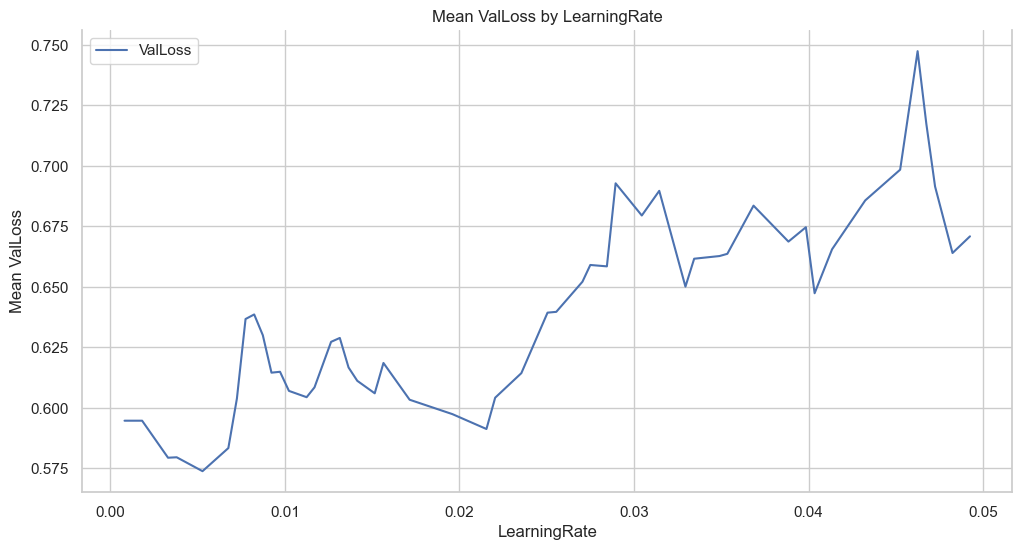
\includegraphics[width=0.6\textwidth]{figures/06_ModelExploration/RNN/rnn_learning_rate.png}
    \caption{Evaluation of the RNN's learning rate with respect to the mean validation loss.}
    \label{fig:rnn_lerning_rate}
\end{figure}

\section{Further Material on the Performance of the MOE Methods}
\label{app:sec:FurtherMOE}

This section provides histogram plots for each introduced \gls{moe} method. These plots depict the density estimates
of the true, under-, and overestimated model orders for the different \gls{snr} metrics-\( \SNRmin \), \( \SIR \), and \( \SNRmax \).
Each figure is divided into two subplots: The upper plot depicts the sample densities of three classes (correct, under-, and overestimated) of all samples in \( \DMain_{(\text{test})} \), while the
lower plot showcases the subset of \( \DMain_{(\text{test})} \) with \( N \leq 3 \). Each histogram consists of 100 bins.


\begin{figure}[H]
    \centering
    \subfloat[\( N \leq 5 \)]{{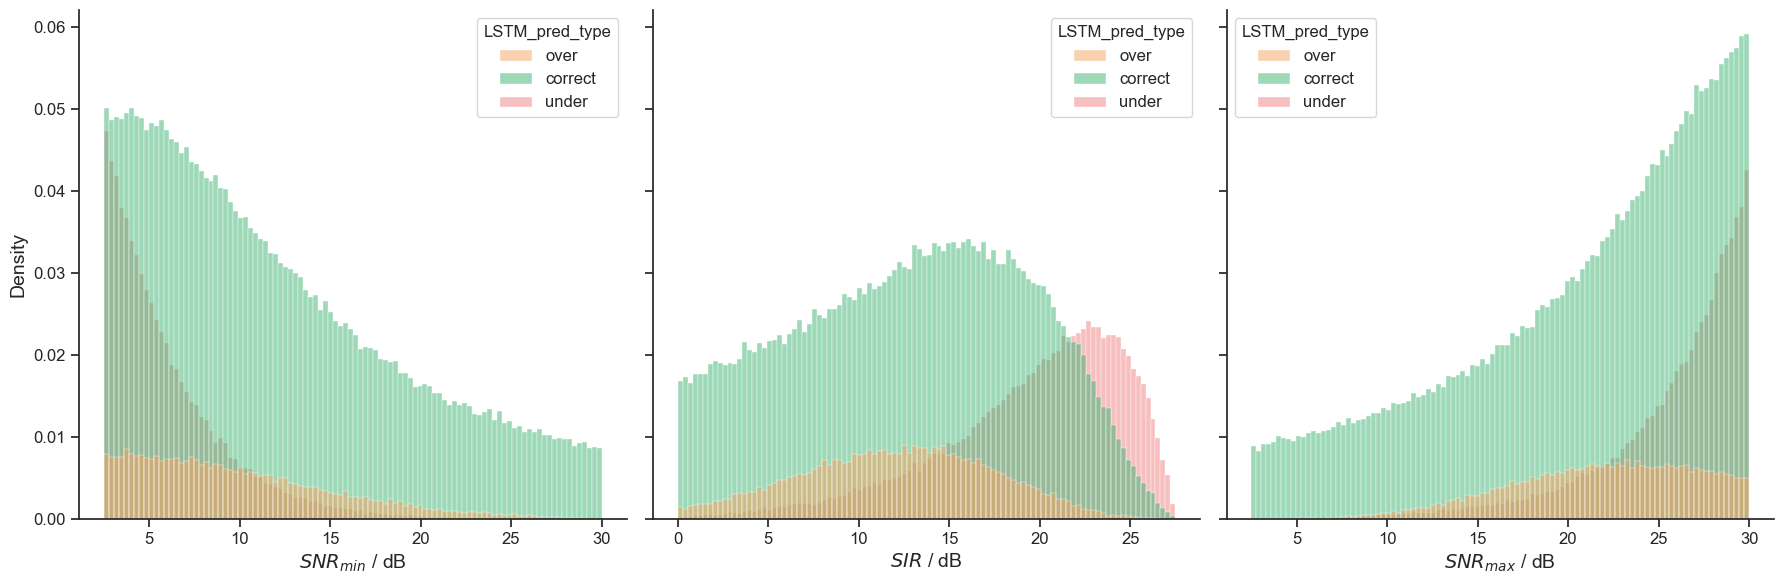
\includegraphics[width=0.9\textwidth]{figures/07_Evaluation/snr_sir/hist/all/lstm.png}}}
    \\
    \subfloat[\( N \leq 3 \)]{{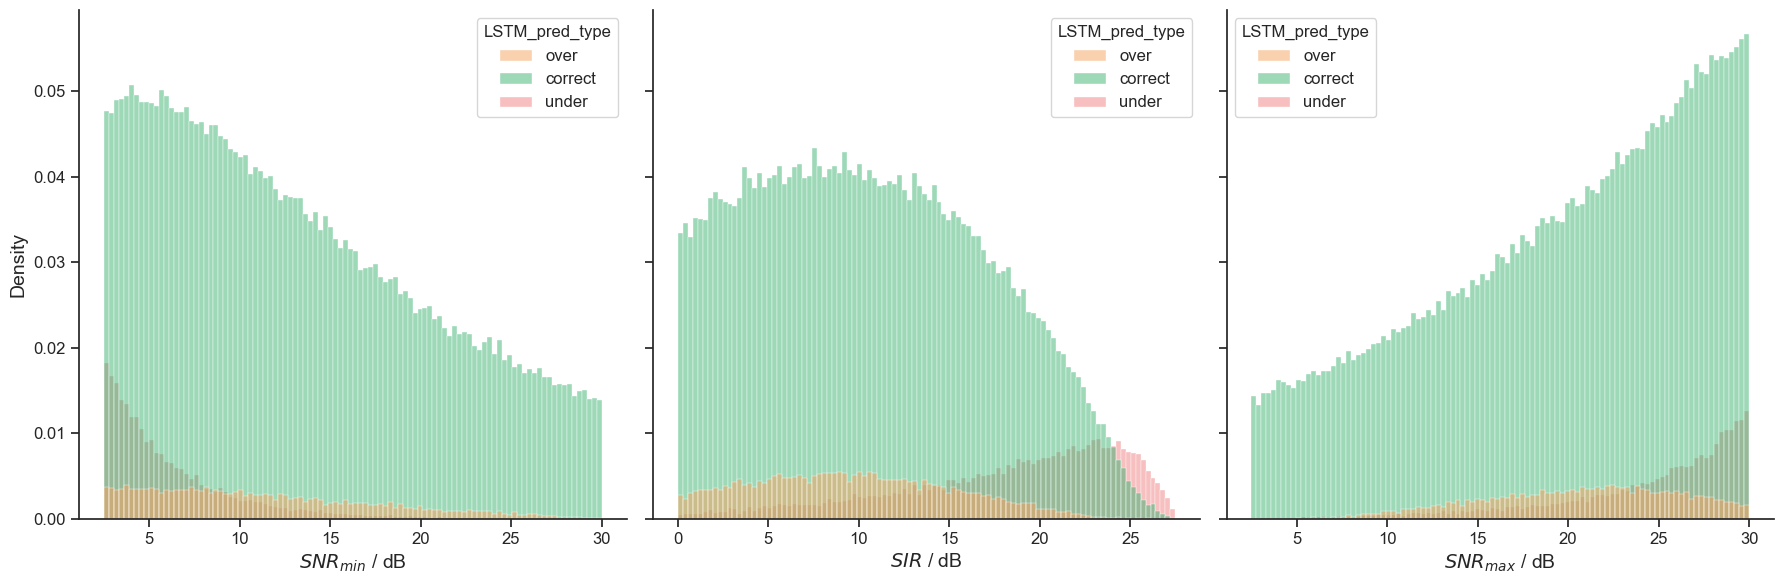
\includegraphics[width=0.9\textwidth]{figures/07_Evaluation/snr_sir/hist/leq3/lstm.png}}}
    \caption{\( \SNRmin \), \( \SIR \), \( \SNRmax \) histograms for LSTM.}
    \label{fig:lstm_pred_hist}
\end{figure}

\begin{figure}[H]
    \centering
    \subfloat[\( N \leq 5 \)]{{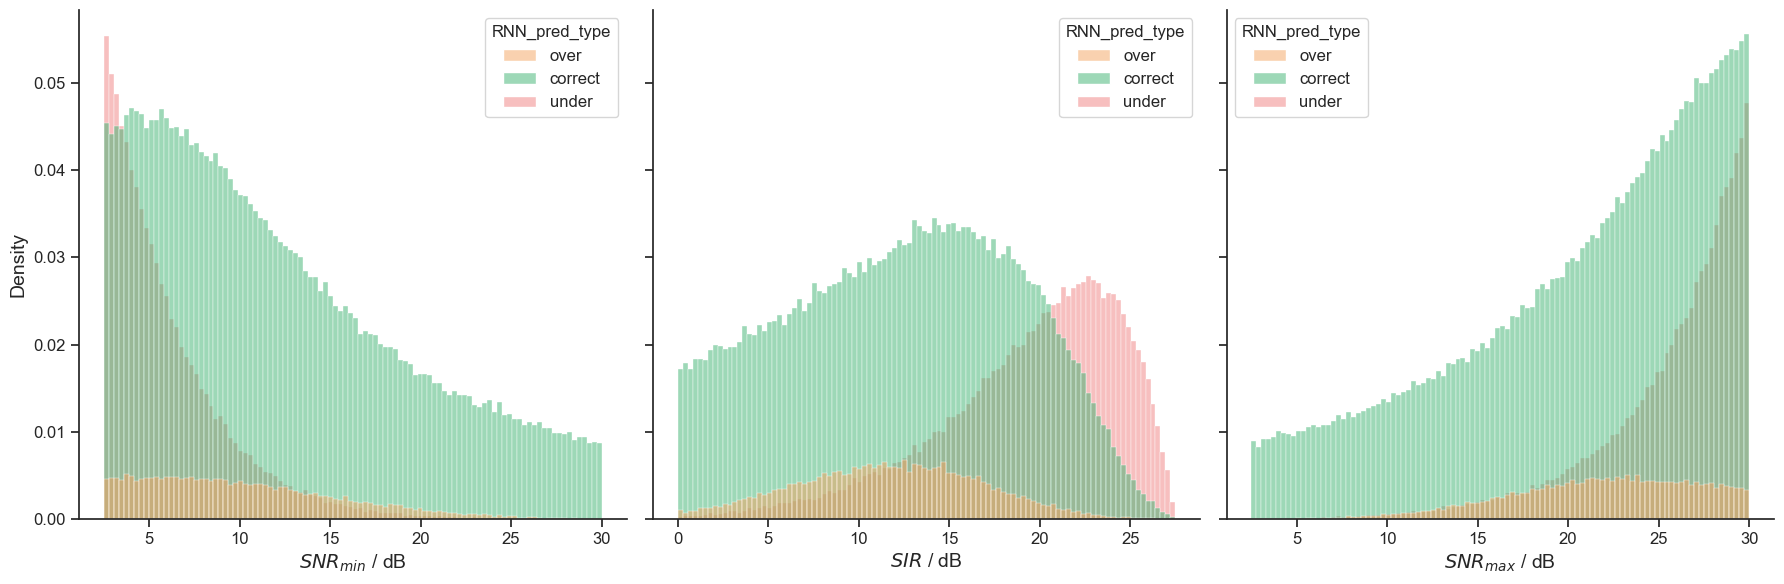
\includegraphics[width=0.9\textwidth]{figures/07_Evaluation/snr_sir/hist/all/rnn.png}}}
    \\
    \subfloat[\( N \leq 3 \)]{{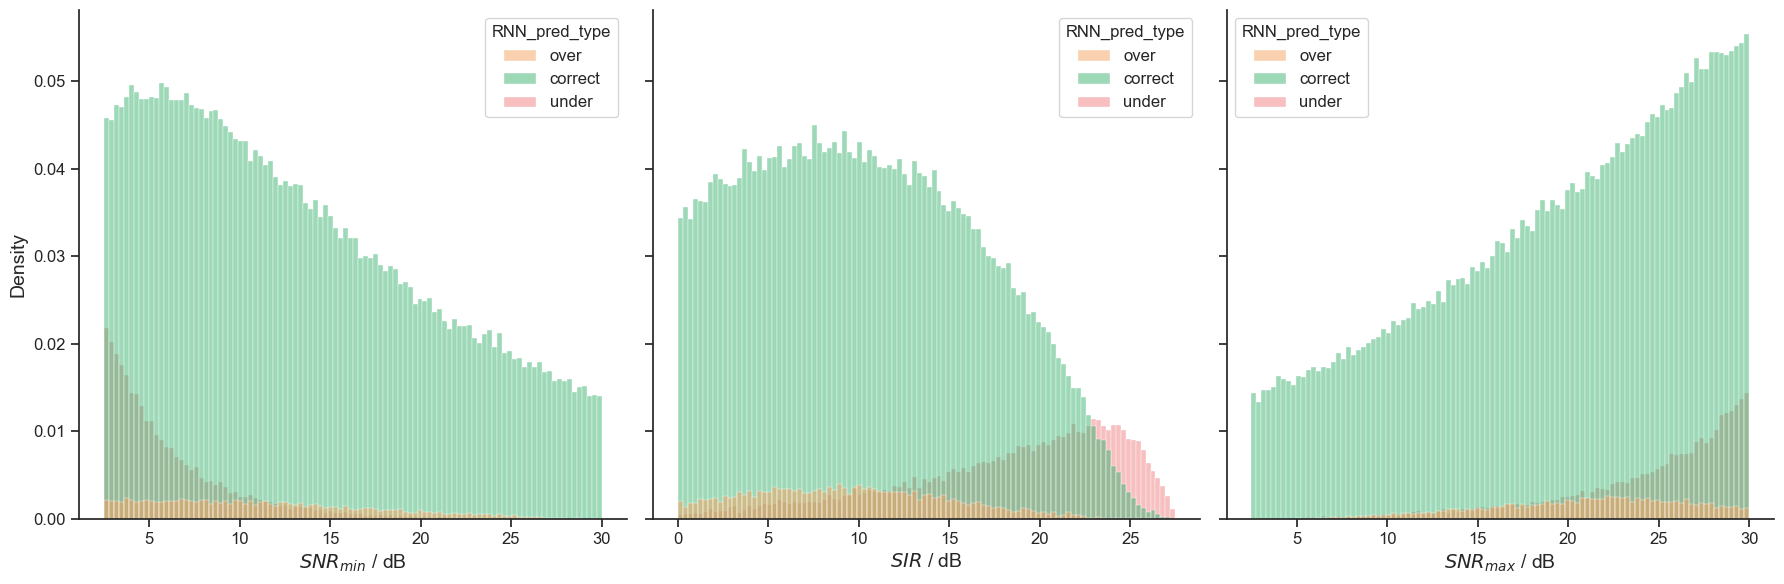
\includegraphics[width=0.9\textwidth]{figures/07_Evaluation/snr_sir/hist/leq3/rnn.png}}}
    \caption{\( \SNRmin \), \( \SIR \), \( \SNRmax \) histograms for RNN.}
    \label{fig:rnn_pred_hist}
\end{figure}

\begin{figure}[H]
    \centering
    \subfloat[\( N \leq 5 \)]{{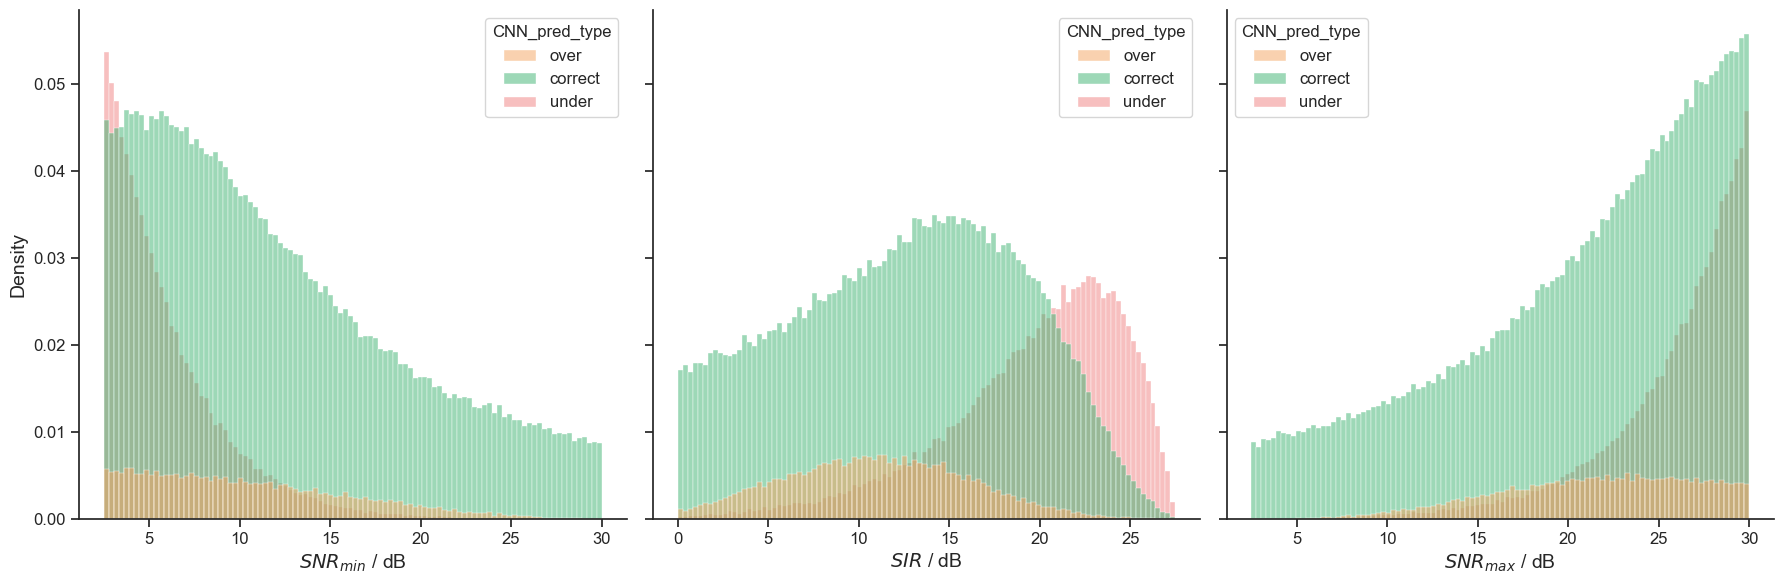
\includegraphics[width=0.9\textwidth]{figures/07_Evaluation/snr_sir/hist/all/cnn.png}}}
    \\
    \subfloat[\( N \leq 3 \)]{{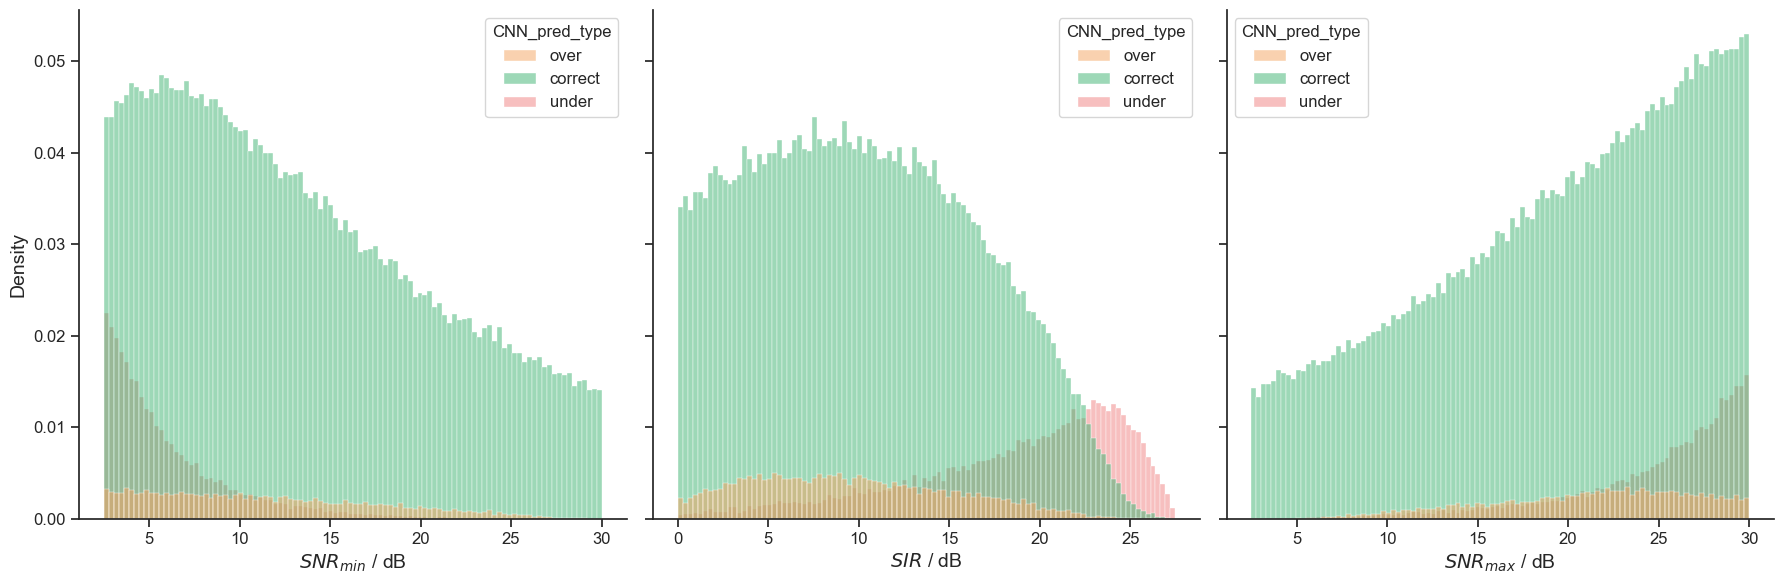
\includegraphics[width=0.9\textwidth]{figures/07_Evaluation/snr_sir/hist/leq3/cnn.png}}}
    \caption{\( \SNRmin \), \( \SIR \), \( \SNRmax \) histograms for CNN.}
    \label{fig:cnn_pred_hist}
\end{figure}

\begin{figure}[H]
    \centering
    \subfloat[\( N \leq 5 \)]{{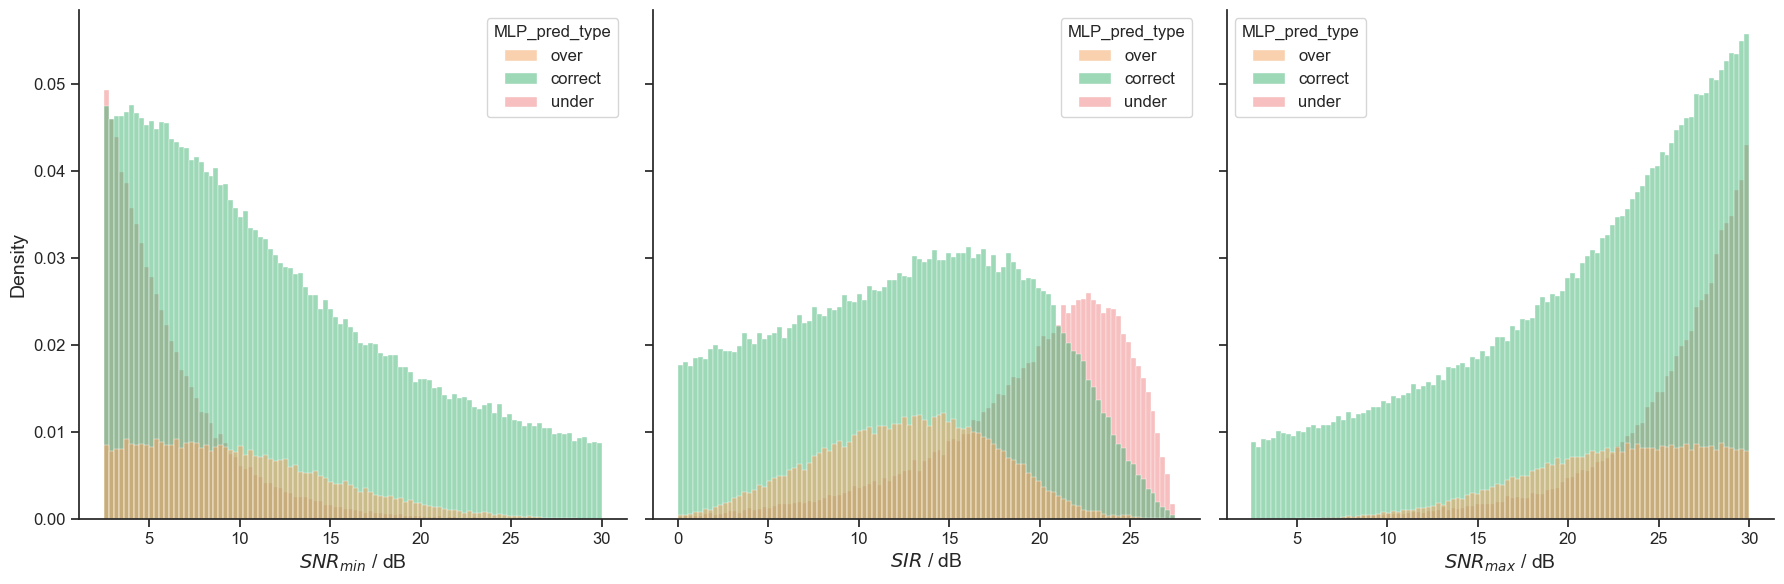
\includegraphics[width=0.9\textwidth]{figures/07_Evaluation/snr_sir/hist/all/mlp.png}}}
    \\
    \subfloat[\( N \leq 3 \)]{{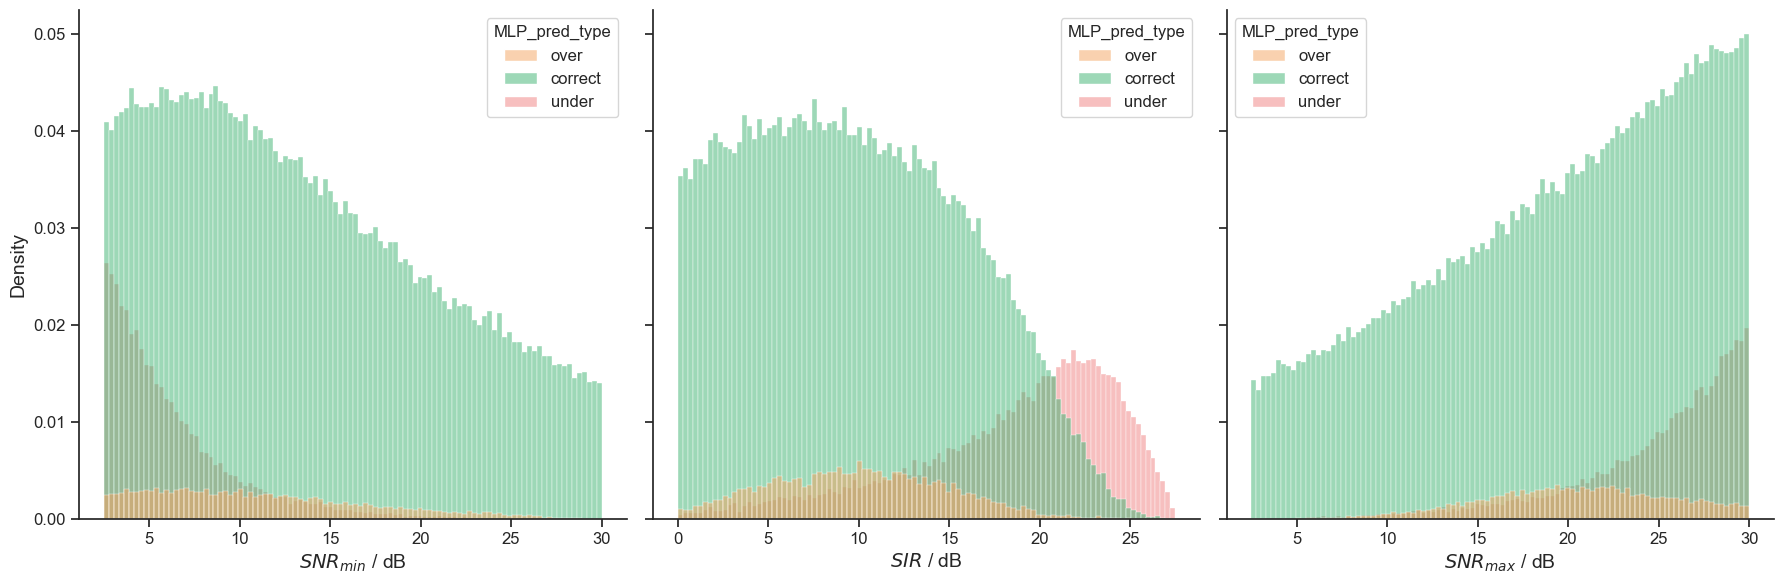
\includegraphics[width=0.9\textwidth]{figures/07_Evaluation/snr_sir/hist/leq3/mlp.png}}}
    \caption{\( \SNRmin \), \( \SIR \), \( \SNRmax \) histograms for MLP.}
    \label{fig:mlp_pred_hist}
\end{figure}

\begin{figure}[H]
    \centering
    \subfloat[\( N \leq 5 \)]{{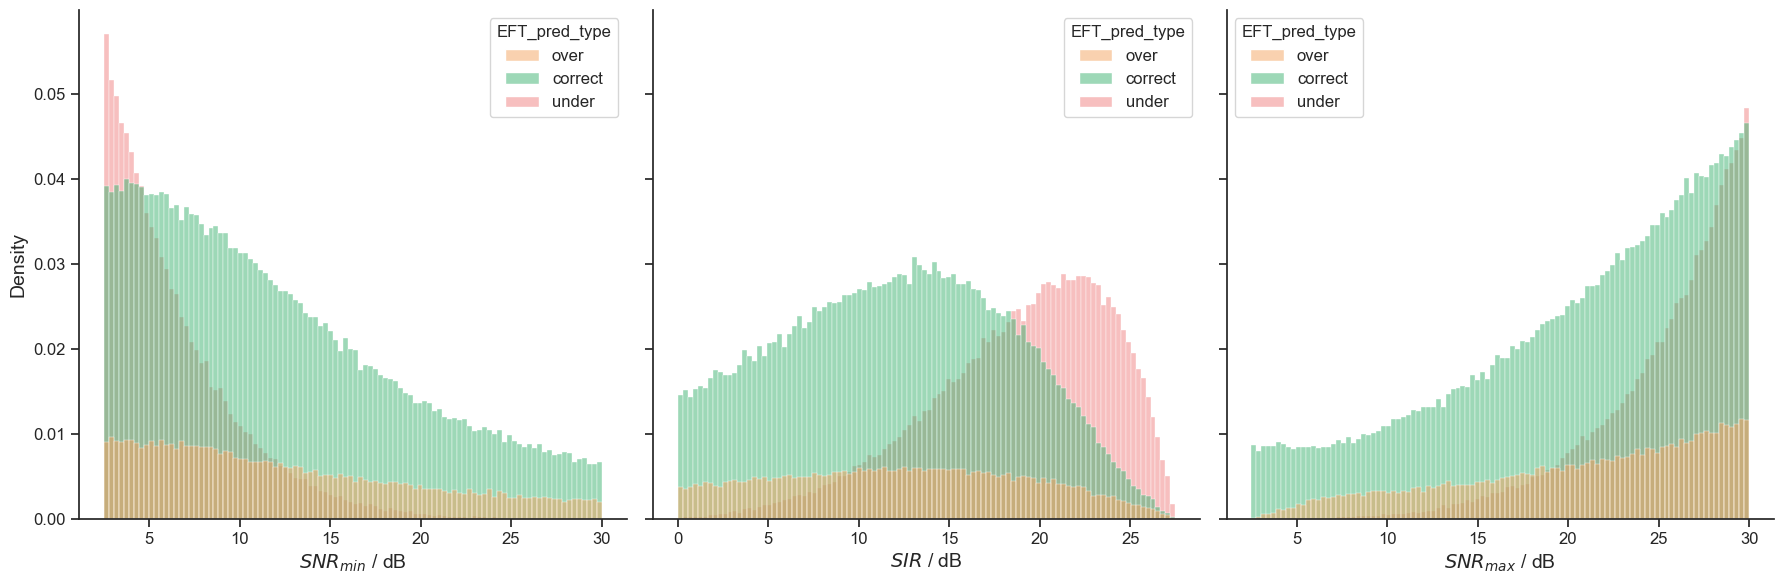
\includegraphics[width=0.9\textwidth]{figures/07_Evaluation/snr_sir/hist/all/eft.png}}}
    \\
    \subfloat[\( N \leq 3 \)]{{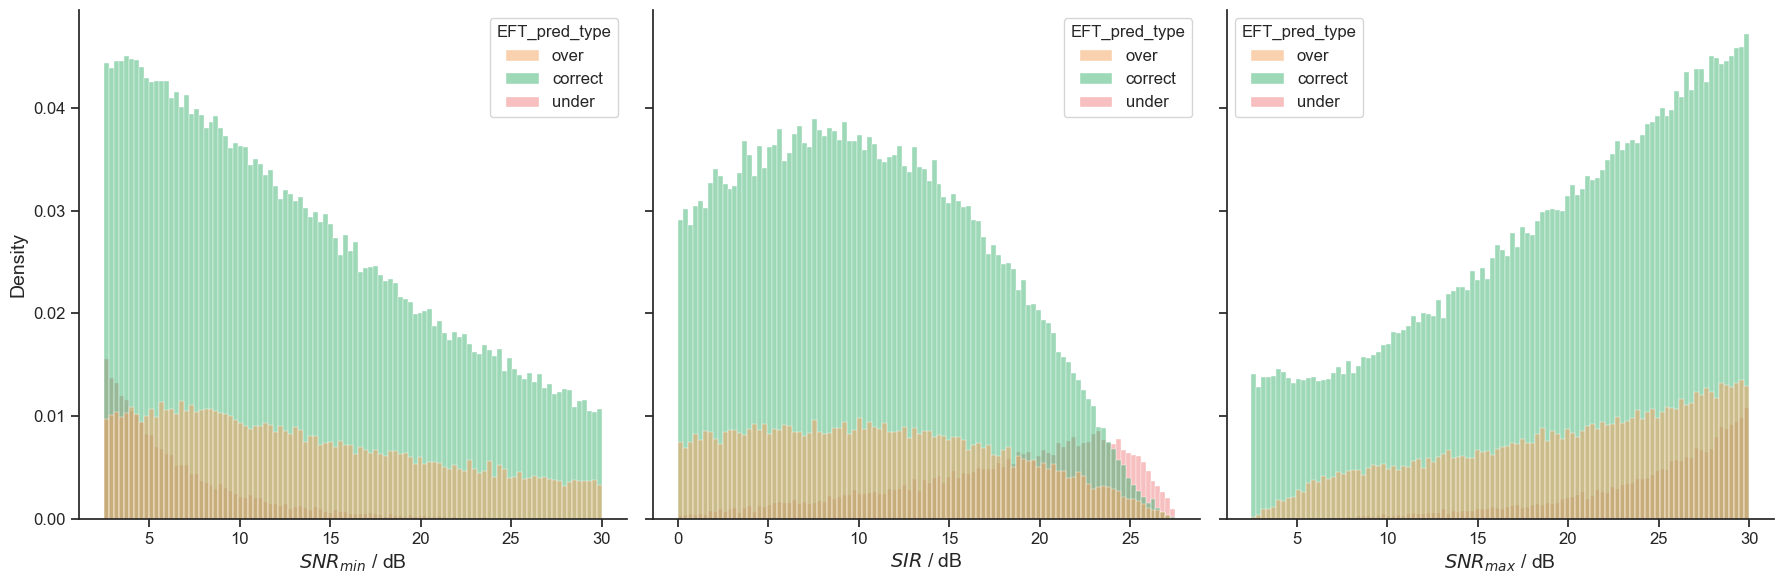
\includegraphics[width=0.9\textwidth]{figures/07_Evaluation/snr_sir/hist/leq3/eft.png}}}
    \caption{\( \SNRmin \), \( \SIR \), \( \SNRmax \) histograms for EFT.}
    \label{fig:eft_pred_hist}
\end{figure}

\begin{figure}[H]
    \centering
    \subfloat[\( N \leq 5 \)]{{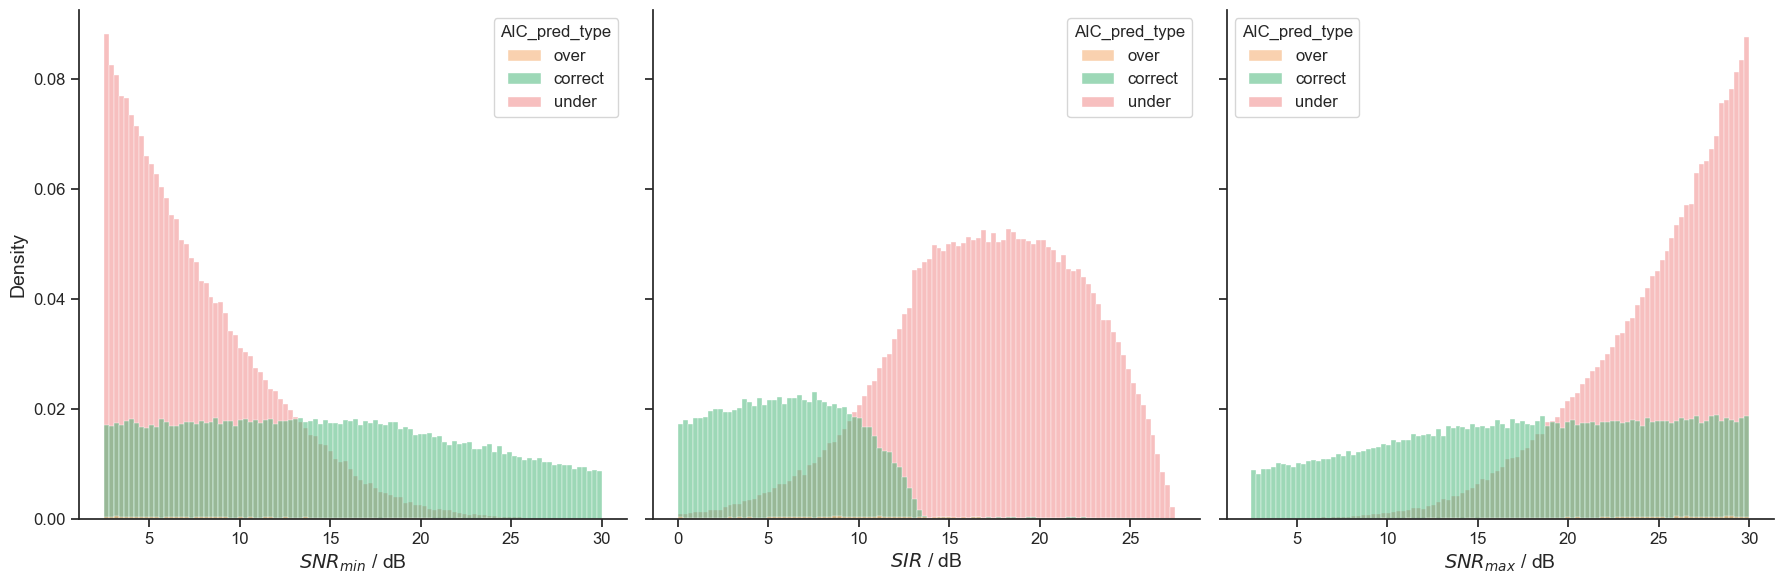
\includegraphics[width=0.9\textwidth]{figures/07_Evaluation/snr_sir/hist/all/aic.png}}}
    \\
    \subfloat[\( N \leq 3 \)]{{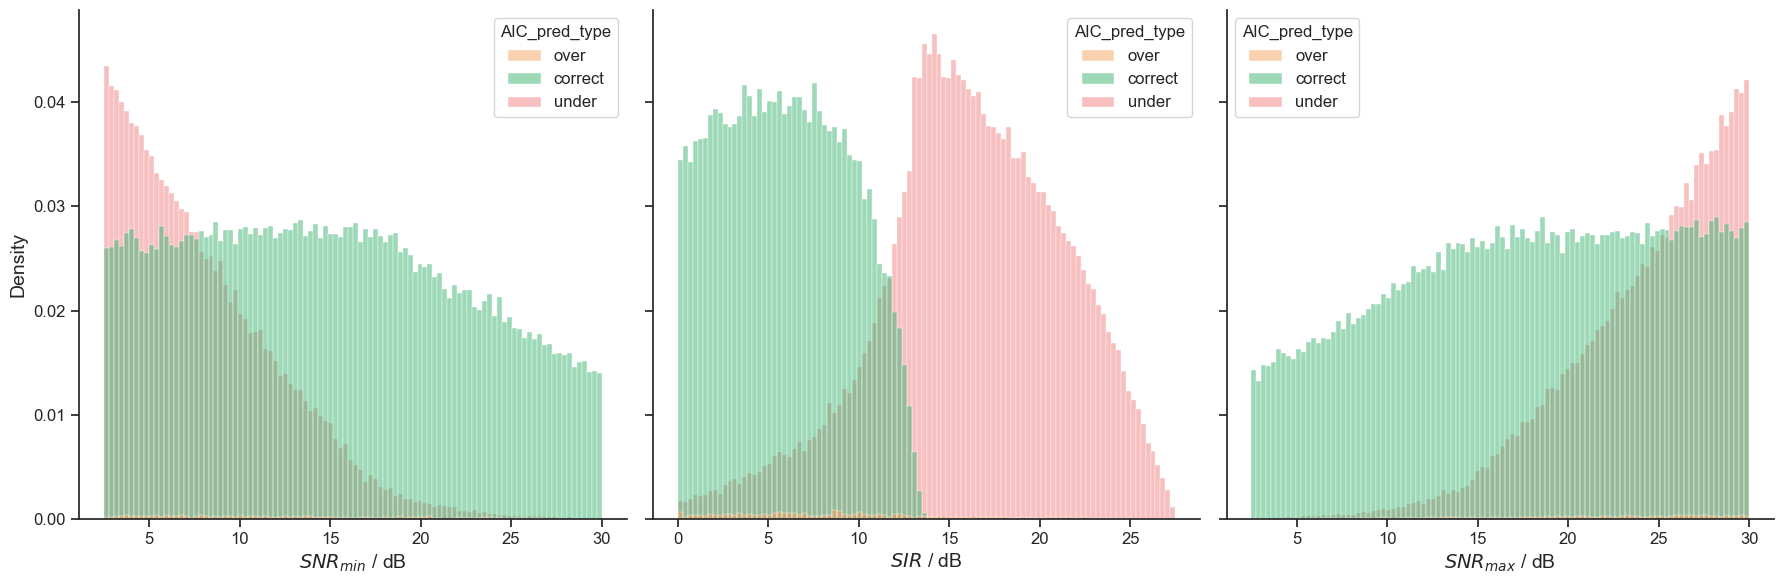
\includegraphics[width=0.9\textwidth]{figures/07_Evaluation/snr_sir/hist/leq3/aic.png}}}
    \caption{\( \SNRmin \), \( \SIR \), \( \SNRmax \) histograms for AIC.}
    \label{fig:aic_pred_hist}
\end{figure}


\begin{figure}[H]
    \centering
    \subfloat[\( N \leq 5 \)]{{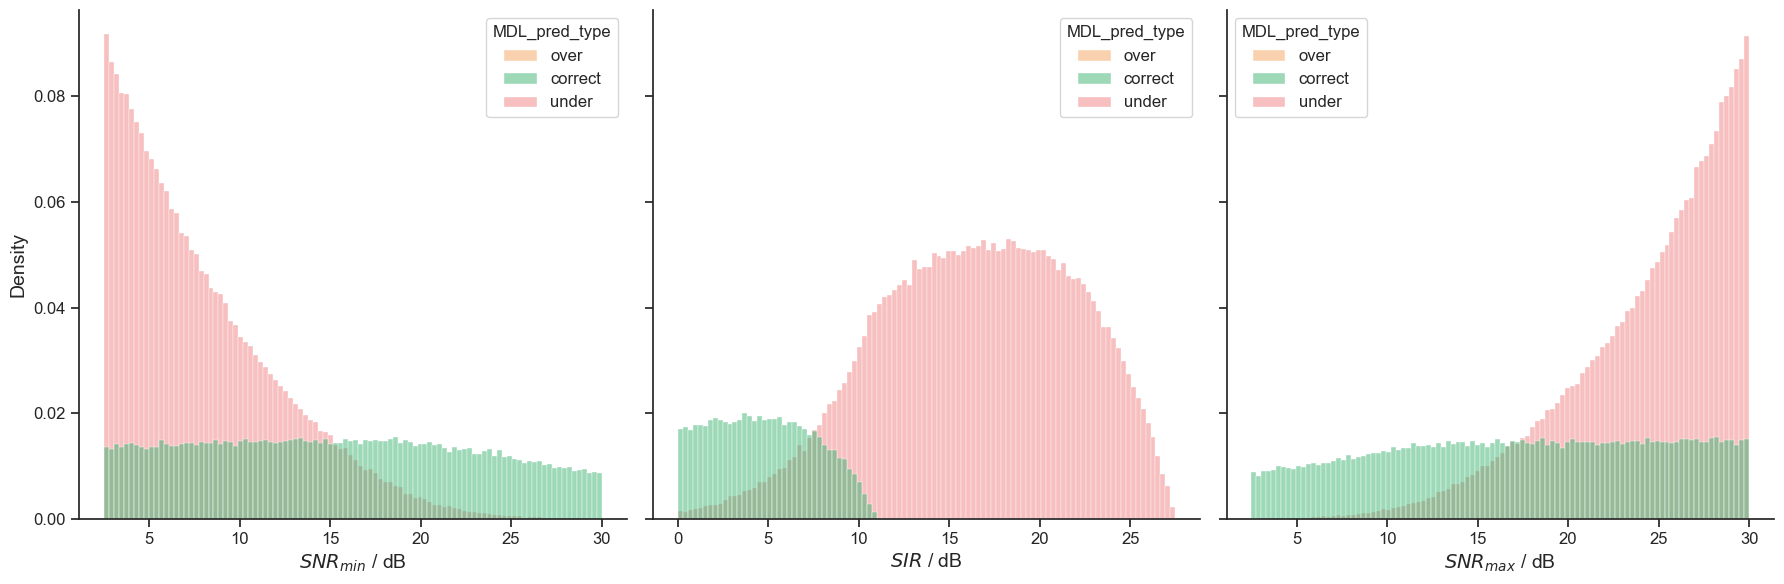
\includegraphics[width=0.9\textwidth]{figures/07_Evaluation/snr_sir/hist/all/mdl.png}}}
    \\
    \subfloat[\( N \leq 3 \)]{{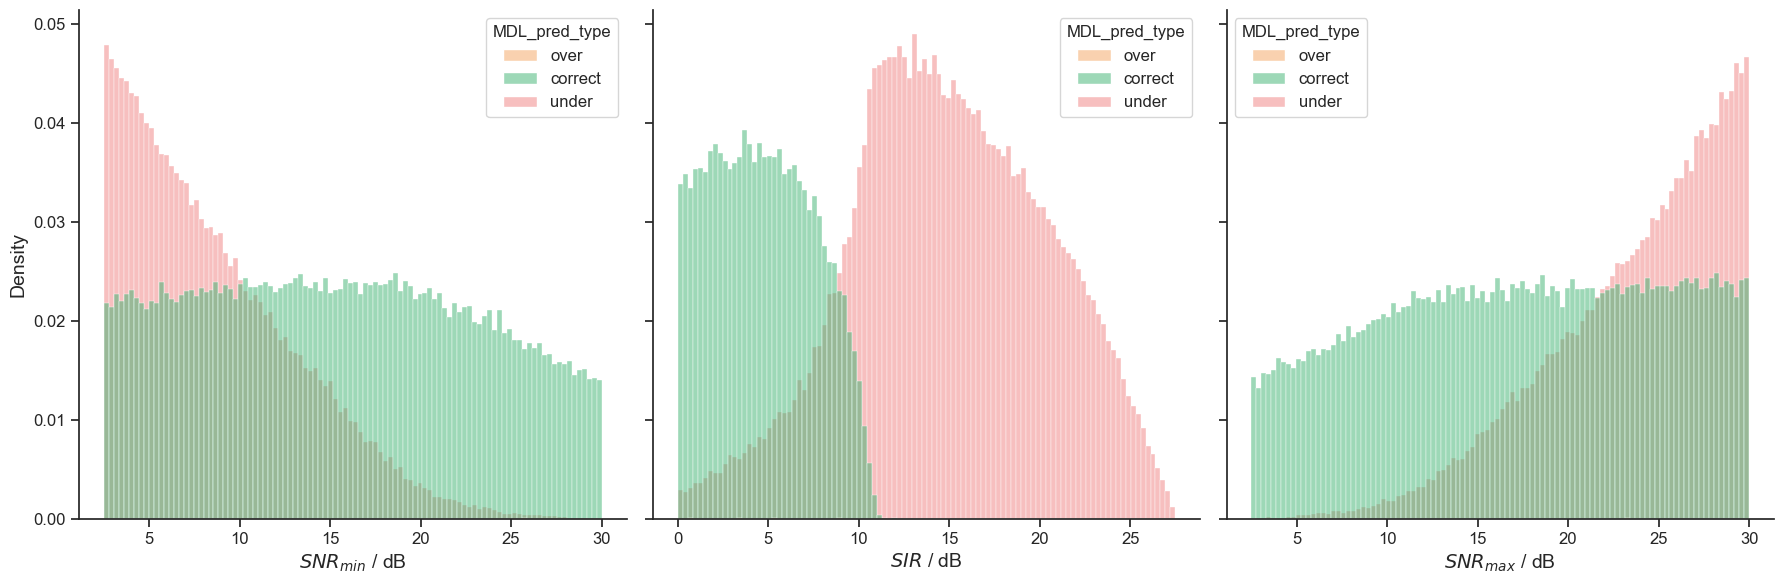
\includegraphics[width=0.9\textwidth]{figures/07_Evaluation/snr_sir/hist/leq3/mdl.png}}}
    \caption{\( \SNRmin \), \( \SIR \), \( \SNRmax \) histograms for \gls{mdl}.}
    \label{fig:mdl_pred_hist}
\end{figure}

